\section{Einleitung}

\subsection{Informationstheorie}

Bit: binary unit $\rightarrow$ Einheit für Information

bit: binary digit $\rightarrow$ bit als binäres Symbol

\textbf{Informationgehalt} 

je unwahrscheinlicher ein Symbol $x$ auftritt, desto mehr Information enhält es:

$\displaystyle{
    I(x) = ld\left( \frac{1}{P(x)} \right) -ld(P(x))
}$

$P$: Wahrscheinlichkeit eines Symbols\\
$I$: Informationsgehalt $[I] = Bit$

\textbf{Entropie}

gemittelter Informationsgehalt einer Quelle $X$:

$\displaystyle{
    H(X) = \sum_{i} P(x_i) \cdot I(x_i) = - \sum_{i} P(x_i) \cdot ld(P(x_i))
}$

$H$: Entropie $[H] = Bit/Symbol$

\textbf{Entscheidungsgehalt}

Entropie wird maximal, wenn alle Symbole gleichwahrscheinlich sind
$\rightarrow$ Entscheidungsgehalt

$\displaystyle{
    H_0 = ld(N)
}$

$H_0$: Entscheidungsgehalt $[H_0] = Bit/Symbol$\\
$N$: Anzahl der Symbole eines Alphabets

\textbf{Redundanz}

$\displaystyle{
    R = H_0 - H
}$

$\displaystyle{
    r = \frac{R}{H_0}
}$

$R$: Redundanz $[R] = Bit/Symbol$\\
$r$: relative Redundanz

%%//TODO: mittlere Laenge Code

\subsection{Quellcodierung}

\subsubsection{Huffman-Code}

ist \textbf{Präfixcode:} ein Codewort ist niemals Anfang eines anderen Codewortes

Codebaum aufbauen:
\begin{enumerate}
    \item Ordne die Symbole nach Auftrittswahrscheinlichkeit
    \item Fasse Symbole mit niedrigster Wahrscheinlichkeit zu einem Symbol zusammen und addiere die Wahrscheinlichkeiten
    \item Wiederhole bis nur ein Symbol übrig bleibt
\end{enumerate}

Beschrifte die Pfade mit 1 und 0\\
$\rightarrow$ Codewort ergibt sich, indem man von Wurzel bis zum Blatt geht

%%// TODO: beispiel rein

\subsubsection{Arithmetische Codierung}

Codierung eines Wortes (oder Textes) durch Zahl

Endezeichen notwendig, da keine natürliche Terminierung des Codes

\subsection{Kanalmodell}

\subsection{Kanalkapazität}

\subsection{Shannon-Theoreme}

\section{Blockcodes}

Code beschrieben durch $C(n, k, d)$

$n$: Länge Codewort\\
$k$: Länge Informationswort\\
$d$: Mindestabstand

\section{Galois-Felder}
\label{sec:galois}

\subsection{Algebraische Strukturen}

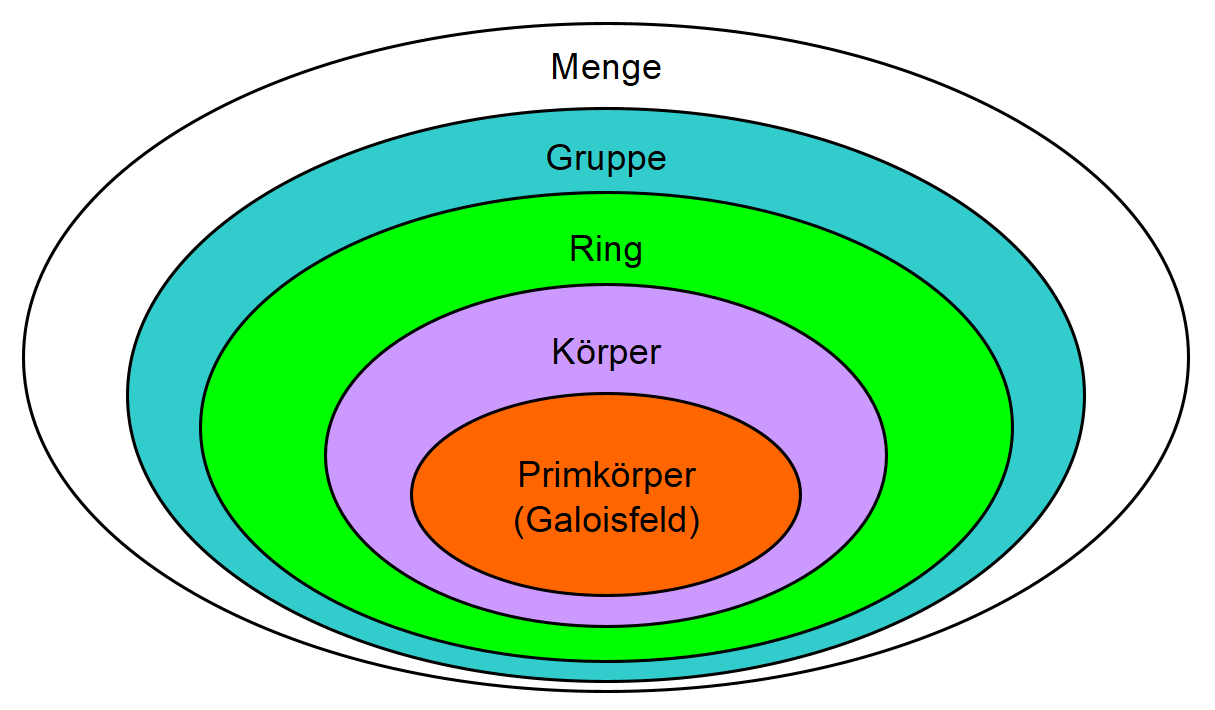
\includegraphics[width=8cm]{img/algebraische_strukturen.PNG}

\textbf{Menge}

Verbund von Elementen, welche keine Operationen beinhalten (Möbel können eine Menge sein, es kann aber nicht Tisch + Stuhl gerechnet werden)

\textbf{Halbgruppe}

Menge $A$ mit Verknüpfung \frqq +\flqq{} ist eine Halbgruppe, wenn
\begin{itemize}
    \item Abgeschlossenheit (+ zweier Elemente von $A$ ergibt wieder ein Element von $A$)
    \item Assoziativität (Reihenfolge der Operation mit + spielt keine Rolle, $a + (b + c) = (a + b) + c$)
    \item Existenz eines neutralen Elements (Element $a$ + neutrales Element $n$ ergibt wieder Element $a$)
\end{itemize}

\textbf{Gruppe}

Halbgruppe plus
\begin{itemize}
    \item Existenz eines additiven inversen Elements ($a + b = n$)
\end{itemize}

\textbf{Abelsche oder kommutative Gruppe}

Gruppe plus
\begin{itemize}
    \item Kommutativität (Reihenfolge der Operanden spielt keine Rolle, $a + b = b + a$)
\end{itemize}

\textbf{Ring}

abelsche Gruppe plus
\begin{itemize}
    \item Abgeschlossenheit bezüglich \frqq $\cdot$\flqq
    \item Assoziativität bezüglich \frqq $\cdot$\flqq
    \item Distributivität ($a \cdot (b + c) = a \cdot b + a \cdot c$)
\end{itemize}

\textbf{Körper}

Ring plus
\begin{itemize}
    \item Kommutativität bezüglich \frqq $\cdot$\flqq ($a \cdot b = b \cdot a$)
    \item Neutrales Element bezüglich \frqq $\cdot$\flqq
    \item Inverses Element bezüglich \frqq $\cdot$\flqq für jedes Element
\end{itemize}

\textbf{Primkörper/Galois-Feld}

Körper, indem Addition und Multiplikation $\mod p$ gerechnet wird ($p$ muss dabei eine Primzahl sein)\\
$\hookrightarrow GF(p)$

\subsection{Eigenschaften Galois-Felder}

\textbf{Primitives Element}

Element $\alpha$, welches durch ihre $p-1$ Potenzen alle Elemente (außer $0$) des $GF(p)$ erzeugt

Bsp. $GF(5), \alpha = 2$:

$2^0 = 1 \mod 5 = 1$\\
$2^1 = 2 \mod 5 = 2$\\
$2^2 = 4 \mod 5 = 4$\\
$ 2^3 = 8 \mod 5 = 3$

ab hier zykische Wiederholung:\\
$2^4 = 16 \mod 5 = 1$

%%//TODO: DFT, zyklische Faltung

\section{Reed-Solomon-Code}

\subsection{Wunsch und Idee}

\textbf{Wunsch}

Konstruktion eines Codes mit vorgegebener Korrekturfähigkeit\\
$\rightarrow$ Vorgabe des Mindestabstandes $d$

$\displaystyle{
    e = \Bigl\lfloor \frac{d - 1}{2} \Bigr\rfloor
}$\\
$\displaystyle{
    d = 2e - 1
}$

bei linearem Code ist Mindestabstand = Mindestgewicht

$\rightarrow$ Codeworte haben mind. $d$ von 0 verschiedene Koeffizienten

d'Alembert: Polynom vom Grad $n$ hat $n$ komplexe (oder höchstens $n$ reelle) Nullstellen; auch
im Galois-Feld

\textbf{Idee}

Konstruktion des Informationswortes als Polynom $A(x)$ mit Grad $k-1$ (damit höchstens $k-1$ Nullstellen)

Im $GF(p)$ mit Ordnung $n = p-1$ kann man $A(x)$ an $n$ Stellen auswerten, danach wiederholen sich die Werte

$\rightarrow$ Auswertung des Polynoms für verschiedene $x$ (bzw. $\alpha^i$) ergeben die Koeffizienten $a_i$ des
Polynoms $a(x)$

$\displaystyle{
    a_i = A(\alpha^i) \qquad\qquad \text{IDFT}
}$

von diesen sind höchstens $k-1$ Null (weil $grad(A(x)) = k-1$)\\
von diesen sind also mind. $n - (k-1)$ von Null verschieden $\rightarrow$ Mindestgewicht $d$

$d = n - (k - 1) = n - k + 1$

\subsection{Codierung}

Verschiedene Möglichkeiten aus einem Informationswort ein Codewort zu generieren

\subsubsection{IDFT (nicht systematisch)}

$\displaystyle{
    a_i = A(\alpha^i)
}$

$A(x)$: Informationswort\\
$a_i$: Koeff. des Codewortes

\subsubsection{Generatorpolynom (nicht systematisch)}

$\displaystyle{
    a_i = g(x) \cdot i(x)
}$

mit Generatorpolynom

$\displaystyle{
    g(x) = \prod_{i=k}^{n-1} \left(x - \alpha^{-i}\right)
}$

$g(x)$: Generatorpolynom\\
$i(x)$: Informationspolynom

\subsubsection{Polynomdivision (systematisch)}

Informationswort ist Teil des Codewortes (an den hohen Potenzen)

$\displaystyle{
    a^*(x) = i_{k-1} x^{n-1} + i_{k-2} x^{n-2} + ... + i_1 x^{n-k+1} + i_0 x^{n-k}
}$

jedes Codewort muss durch Generatorpolynom teilbar sein $\rightarrow$ ist
für $a^*(x)$ i.A. nicht der Fall

$\displaystyle{
    \frac{a^*(x)}{g(x)} = b(x) + \frac{rest(a^*(x))}{g(x)}
}$\\
$\displaystyle{
    \rightarrow \frac{a^*(x) - rest\left(a^*(x)\right)}{g(x)} = b(x)
}$\\
$\displaystyle{
    a(x) = a^*(x) - rest\left(a^*(x)\right)
}$

$rest\left(a^*(x)\right)$: Divisionsrest

\subsubsection{Über Prüfpolynom (systematisch)}

Prüfpolynom:

$\displaystyle{
    h(x) = \prod_{i=0}^{k-1} \left(x - \alpha^{-i}\right)
}$

Produkt aus Generator- und Prüfpolynom ist 0

$\displaystyle{
    g(x) \cdot h(x) = 0
}$

und Produkt aus Codepolynom und Prüfpolynom ist 0

$\displaystyle{
    a(x) \cdot h(x) = 0
}$

genau da, wo $g(x)$ (oder $a(x)$) Nullstellen hat (also $G_i$ 0 ist) hat das Prüfpolynom $h(x)$ keine Nullstellen
(ist also $H_i$ nicht 0) und umgekehrt

\subsection{Decodierung}

\textbf{Idee:}

Addition des Fehlerpolynoms $f(x)$ mit $t$ Koeffizienten (d.h. $t$ Fehler sind auf dem Kanal aufgetreten)
zum gesendeten Codewort $a(x)$

im Zeitbereich:

$\displaystyle{
    r(x) = a(x) + f(x)
}$

im Frequenzbereich:

$\displaystyle{
    R(x) = A(x) + F(x)
}$

gedanklich wird ein Polynom $c(x)$ aufgestellt, welches $t$ Nullen an den Fehlerstellen hat

Da die Koeffizienten von $c(x)$ die Auswertung ihrer Fouriertransformierten $C(x)$ ist, ist der Grad
von $C(x)$ $t$

Da $c(x)$ gerade dort 0 ist, wo $f(x)$ ungleich 0, ist das Produkt $f_i \cdot c_i$ immer 0 (Achtung, keine
Polynommultiplikation gemeint, sondern punktweise Multiplikation)

$\displaystyle{
    f_i \cdot c_i = 0
}$

wenn Zeitbereich = 0 $\rightarrow$ Frequenzbereich = 0

$\displaystyle{
    F(x) \cdot C(x) = 0
}$

Achtung: hier Polynommultiplikation/ Faltung/ Filterung gemeint\\
$\hookrightarrow$ Aufstellen der Schlüsselgleichungen

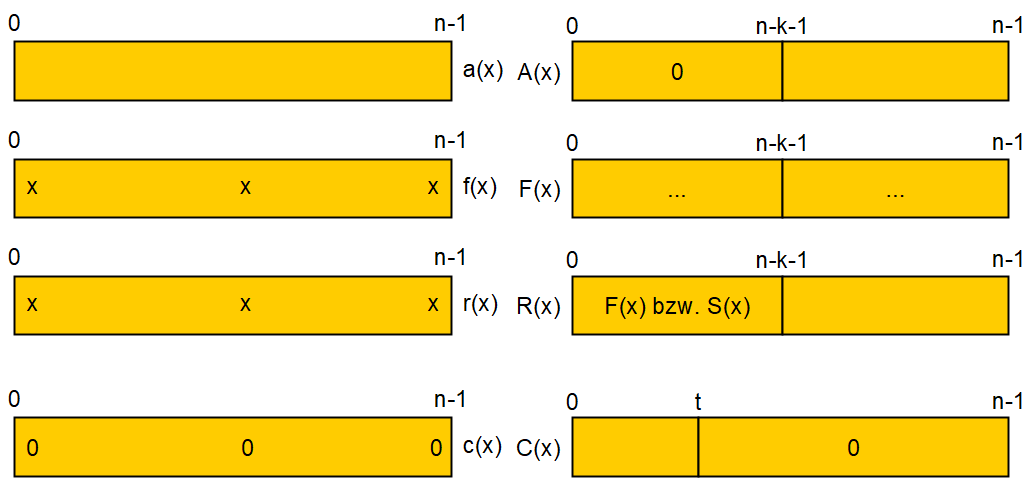
\includegraphics[width=8cm]{img/decod_rs.PNG}

\subsubsection{Schlüsselgleichungen}

beschreiben, dass Faltung von $C(x)$ und $F(x)$ Null ist (Achtung: zyklische Faltung, siehe \autoref{sec:galois})

$F_0$ bis $F_{n-k-1}$ (bzw. $F_{d-2}$) sind bekannt, da diese direkt an den Syndromstellen
von $R(x)$ stehen

Alle $C$-Koeff. sind unbekannt, außer $C_{t}$, dieser wird zu $1$ gesetzt

$\displaystyle{
    C_{t} = 1
}$

da Anzahl der Fehler ($t$) unbekannt ist, muss ausprobiert werden, welche \underline{minimale} Anzahl an Fehlern
die Schlüsselgleichungen widerspruchsfrei erfüllt

Lösen der Schlüsselgleichungen nach $C(x)$

$\hookrightarrow$ Nullstellensuche von $C(x)$ ergibt die Nullen des $c(x)$

$\hookrightarrow$ wenn Grad von $C(x)$ nicht mit Anzahl der Nullstellen übereinstimmt $\rightarrow$ Decodierversagen

Lösen der Schlüsselgleichungen nach $F(x)$

$\hookrightarrow f(x)$ aus Rücktransformation von $F(x)$

$\hookrightarrow f(x)$ von $r(x)$ abziehen, man erhält $a(x)$

$\displaystyle{
    a(x) = r(x) - f(x)
}$

%%// TODO: Schlüsselgleichungen aufstellen

\textbf{Berlekamp-Massey-Algorithmus}

effizientes Verfahren zur Lösung der Schlüsselgleichungen

%%//TODO

\textbf{Euklidscher Algorithmus}

Suche des ggT zweier Zahlen

Kann zur Lösung der Schlüsselgleichungen verwendet werden

%%// TODO

\subsection{Horner-Schema}

\section{Erweiterungskörper}

Erweitern des Grundkörpers (z.B. $2$) mit Exponent (z.B. $4$) $\rightarrow$
$GF(2^4)$

primitives Element wird zu primitivem Polynom, z.B.
$\displaystyle{
    p(x) = x^4 + x + 1
}$

\section{BCH-Codes}

